\documentclass{article}

\usepackage[utf8]{inputenc}
\usepackage[T1]{fontenc}
\usepackage{lipsum}
\usepackage{graphicx}
\usepackage{amsmath}
\usepackage[margin=1in]{geometry}
\usepackage{titlesec}
\usepackage{enumitem}

\titleformat{\section}
{\LARGE\bfseries}{\thesection}{1em}{}

\titleformat{\subsection}
{\Large\bfseries}{\thesection}{1em}{}

\begin{document}
\pagestyle{empty}
\section*{Design pattern}
\large

\subsection*{Introduzione}
\large
Obiettivi:
\begin{itemize}
    \renewcommand{\labelitemi}{-}
    \itemsep0em
    \item Applicare propriamente i pattern del modello GoF 
\end{itemize}
Prima di introdurre i particolari dei pattern del modello GoF, si definiscono le lucidazioni necessarie per comprendere l'etimologia del termine.\vspace*{14pt}\\
\textit{Definizione informale}\\
Ogni pattern descrive uno specifico problema e la sua soluzione associata, per fare in modo che la soluzione possa essere ripetuta anche in nuovi contesti del modello.\vspace*{14pt}\\
Riassumendo il contesto, l'intento consiste nella decodifica dell'esperienza vissuta, affinchè ciò che è stato riscontrato possa essere adeguato in altri contesti. Esistono tante altre definizioni del termine, ma basti pensare alla correlazione diretta presente tra la denominazione del problema e della soluzione, pur di ottenere l'idea su cui fonda un pattern.\vspace*{14pt}\\
Spesso i \textit{pattern} sono raggruppati in strutture coese, ossia accomunate da stesse caratteristiche, le quali danno vita a vocabolari capaci di esprimerne la \textit{sintassi} e la \textit{grammatica}, oppure, a titolo semplificativo, il \textit{contesto} e il \textit{caso d'uso}. Tuttavia, sono presenti un numero elevatissimo di cataloghi inerenti ai pattern applicati in ingegneria del software, ma in questa sezione verrà adoperato il \textit{vocabolario} posto dalla \textit{Gang of Four}.

\subsection*{GoF}
\large
Stabilita un'introduzione al contesto cardine della sezione, si approccia nel dettaglio ciò che contraddistingue maggiormente l'insieme dei pattern del \textit{catalogo GoF}. I pattern caratterizzati si suddividono in tre macro areee, poste come segue:
\begin{itemize}[label={-}]
    \itemsep0em
    \item \textit{Creational}, ...
    \item \textit{Structural}, ... 
    \item \textit{Behavioral}, ... 
\end{itemize} 
Tuttavia, prima di illustrare nel dettaglio tutti i pattern di riferimento alle classificazioni precedenti, occorre descrivere una tematica su cui fonda la propria logica il meccanismo \textit{GoF}.\vspace*{14pt}\\
Analizzando nuovamente linguaggi legati al paradigma degli oggetti, per adeguare la soluzione software ad un'elevata \textit{reusability} occorre ottimizzare l'utilizzo di caratteristiche particolari, quali \textit{ereditarietà} e \textit{poliformismo}. Per cui l'obiettivo di un qualsiasi team di sviluppo, consiste nella possibilità di riutilizzare porzioni di codice già attutate per risolvere problemi passati. Ciò è possibile tramite il corretto uso di meccanismi legati alle caratteristiche del linguaggio di programmazione adottato, ma non rappresenta l'unica soluzione.\vspace*{14pt}\\
In questo ambito, inerente al catalogo GoF, è posta la preferenza nell'utilizzo di meccanismi legati alla \textbf{delega}, o meglio definiti di \textbf{composizione}, piuttosto che strumenti correlati ad \textit{inheritance}, pur di aumentare la qualità di riutilizzo. La ragione principale è dovuta dalla maggiore conformità del modello proposto rispetto ad un elevato livello di incapsulamento, in cui oggetti di ogni singola classe possano svolgere un unico compito, ossia siano associati ad un solo \textit{comportamento}. Tuttavia di seguito è proposto un caso di studio che possa dimostrare la maggiore efficacia.\vspace*{14pt}\\
\textit{Caso di studio}\\
All'interno dell'esempio è illustrato un insieme di step che possano evidenziare come l'ereditarietà in certe casistiche non risulti essere una soluzione efficace; proponendo una via alternativa, di maggiore correttezza, dovuta al meccanismo di \textit{delega}.
\begin{center}
    \includegraphics*[width=0.5\textwidth]{foto 1.png}
\end{center}\vspace*{7pt}
Come da raffigurazione, sono presenti un totale di quattro classi software, di cui \textit{Vehicle} risulta essere la superclasse. In tale domain model l'implementazione adeguata propone un metodo generale posto nella classe padre denominato \textit{goTo()}, \textit{ereditato} anche dalle classi figlie le quali attuano uno sviluppo personale a seconda del comportamento che debba essere compiuto, per cui adeguando \textit{poliformismo}.\vspace*{7pt}\\
Nonostante possa apparire una soluzione valida, viola il principio di \textit{Liskov}, il quale ammette che se si dovesse verificare nella soluzione software \textit{needless repetition}, ossia l'azione \textit{copia-incolla} tra classi, come avviene per \textit{AirCraft} e \textit{Drone}, allora rappresenta una mancata visualizzazione di un livello di astrazione nella progettazione adeguata fino ad ora. Ciò comporta all'adozione di un'interfaccia che sia sovrapposta tra \textit{Vehicle} e le classi figlie. 
\begin{center}
    \includegraphics*[width=0.5\textwidth]{foto 2.png}
\end{center}
Un meccanismo simile risulta essere solido fino a quando non sia proposta un'ulteriore funzionalità da sviluppare. Infatti, qualora all'interno della superclasse sia posto un ulteriore metodo che dovrà essere ereditato dalle sottoclassi, quale \textit{notifyDriver()}, dimostrandosi totalmente differente per ogni elemento del modello, qualsiasi livello di astrazione non sarebbe sufficiente per poter rispettare i principi legati al modello GRASP, diminuendo la qualità del codice.
\begin{center}
    \includegraphics*[width=0.5\textwidth]{foto 3.png}
\end{center}\vspace*{7pt}
Concludendo, rispetto a quanto detto prima, sarebbe violato il principio \textit{Open Closed}, il quale ammette che in una qualsiasi classe software possano essere aggiunti metodi ma non modificate funzionalità già esistenti, ciò che non rispetterebbe l'implementazione di \textit{notifyDriver()} in ogni singola sottoclasse.\vspace*{14pt}\\
Osservati i limiti che si potrebbero verificare in un meccanismo legato all'\textit{ereditarietà}, una via risolutiva comprende la nozione di \textit{composizione}. Tramite lo strumento della \textit{delega}, è introdotto un livello di astrazione capace di suddividere le classi legate alla logica algoritmica da classi \textit{concrete}.
\begin{center}
    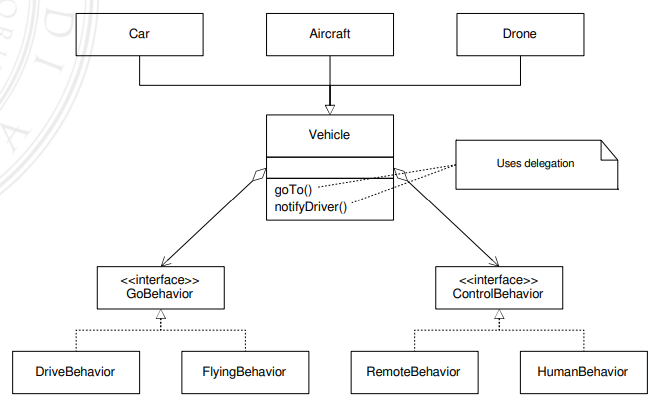
\includegraphics[width=0.7\textwidth]{foto 4.png}
\end{center}\vspace*{7pt}
La raffigurazione ritrae la classe \textit{Vehicle} strettamente connessa all'interfacce \textit{GoBehavior} e \textit{ControlBehavior}, poichè è parte del layer di astrazione; tale scelta è dovuta alla necessità di porre un elemento del modello come mediatore tra l'implementazione dei comportamenti rispetto alle richieste delle classsi derivate. Per cui saranno incapsulate le due istanze delle interfacce all'interno della classe padre, affinchè classi figlie possano reclamare all'interno del costruttore quale implementazione dei metodi \textit{goTo()} e \textit{notifyDriver()} siano necessarie. Si osserva un vero e proprio meccanismo di delega che contraddistingue la \textit{composizione}.\vspace*{14pt}\\
In conclusione, sono riassunti i due punti critici di \textit{inheritance} che comportano alla scelta della \textit{composizione} e del meccanismo della \textit{delega}, quali:
\begin{itemize}[label={-}]
    \itemsep0em
    \item \textit{Poliformismo}, non accetta overriding dei metodi da parte di classi figlie, ciò che è stato già riscontrato all'interno di \textit{Liskov Substitution Principle}. Si ricorda l'affinità con il principio di sotituibilità, il quale ammette che ogni istanza di una sottoclasse sia interpellabile da una superclasse; tuttavia questo non è sufficiente, poichè si richiede anche affinità comportamentale, in cui dovrebbe essere atteso lo stesso comportamento descritto a livelli soprastanti, ossia specifica alla logica logaritmica
    \item \textit{Condivisione comportamentale}, strettamente collegato al punto precedente, in cui pur di implementare metodi comportamentali si aggiungono layer architetturali tra classi padre e classi figlie, illustrando una crescente dissonanza con \textit{behavioral compatibility}
\end{itemize}
Tutto ciò si traduce in azioni mirate che comportino lo spostamento del codice implementato per la rappresentazione di comportamenti al di fuori di contesti dipendenti, inserendo l'implementazione attuata in classi esterne.

\subsection*{Template Method Pattern}
\large
\textit{Problema}\\
Come condividere metodi parzialmente definiti in una gerarchia ereditaria?\vspace*{14pt}\\
\textit{Soluzione}\\
Definire lo schema dell'algoritmo di certe funzionalità, le quali saranno poi specializzate, in base alle necessità, dalle sottoclassi.\vspace*{14pt}\\
\textbf{Template Method} rappresenta uno dei \textit{pattern comportamentali} del \textit{catalogo GoF}, il quale permette di definire la struttura di un algoritmo lasciando alle sottoclassi il compito di implementarne alcuni passi come preferiscono. In questo modo è possibile ridefinire e personalizzare parte del comportamento nelle varie sottoclassi senza dover riscrivere più volte il codice in comune.\vspace*{7pt}\\
E' bene sottolineare che tramite questo meccanismo non avviene overriding dei metodi, anzi la definizione generale della struttura dell'algoritmo permette a classi figlie di implementare solamente step specifici che dovranno essere contraddistinti a seconda del comportamento richiesto.\vspace*{14pt}\\
\textit{Caso di studio}\\
Di seguito è proposto un esempio che prende in considerazione l'effettività di un plotter, suddivisa da due comportamenti specifici adeguati in due sottoclassi sottostanti.
\begin{center}
    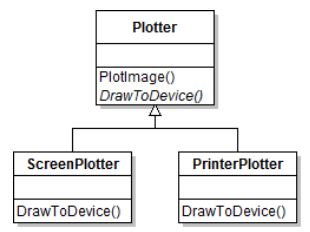
\includegraphics[width=0.4\textwidth]{foto 5.png}
\end{center}\vspace*{7pt}
Come da raffigurazione è rappresentata la classe astratta \textit{Plotter}, la quale definisce lo schema generale dei metodi incapsulati al suo interno. In tale contesto le sottoclassi \textit{ScreenPlotter} e \textit{PrinterPlotter} adeguano il metodo \textit{DrawToDevice()}, specializzando mirate funzionalità affinchè il comportamento sia conforme con le finalità comportamentali, ovviando all'overriding dell'intero metodo.\vspace*{7pt}\\
Tramite tale approccio è ovviato il design smell \textit{needless repetition}, per cui rispettando appieno il principio di \textit{Liskov}, rendendo l'architettura resistente ai cambiamenti.

\subsection*{Strategy Pattern}
\large
\textit{Problema}\\
Come separare un oggetto dal proprio comportamento e variarlo durante il run time?\vspace*{7pt}\\
\textit{Soluzione}\\
Definire un insieme di algoritmi, i quali risultino incapsulati, affinchè siano intercambiali durante il run time.\vspace*{14pt}\\
\textbf{Strategy} per certi aspetti è molto simile al pattern presentato nella sezione precedente, in cui vige una differenza sostanziale. In \textit{Method Template} è definita la struttura generale dell'algoritmo affinchè classi figlie possano specializzare il comportamento a seconda della necessità, mentre in \textit{Strategy} non avviene un meccanismo di suddivisione comportamentale, pone un livello astratto, tipicamente un'interfaccia, da cui saranno estesi \textit{behavior} specifici i quali potranno essere richiamati dalla classe concreta.\vspace*{14pt}\\
\textit{Casi di studio}\\
\begin{center}
    
\includegraphics[width=0.6\textwidth]{foto 6.png}
\end{center}
In questo esempio la classe \textit{Context} mantenendo al suo interno istanze dell'interfaccia che implementa i comportamenti specifici, è in grado di richiamare il \textit{behavior} che più si addice al contesto in cui è posta. Grazie a \textit{Strategy}, è preferita la \textit{composizione} rispetto all'\textit{ereditarietà}, favorendo dinamicità anche durante fasi di run time; dato che i comportamenti derivano dalla stessa interfaccia, la classe \textit{Context}, imponendo attributi differenti, è in grado di intercambiare i metodi messi a disposizione.\vspace*{7pt}\\
In conclusione un caso di studio simile rispetta il principio \textit{Open Closed}, ossia non promuove la modifica di funzionalità già esistenti ma introduce nuove classi che possano implementare i comportamenti desiderati.
\end{document}